\documentclass[11pt, a4paper]{article}
\usepackage[utf8]{inputenc}
\usepackage[italian]{babel}
\usepackage{amsmath, amssymb}
\usepackage{geometry}
\usepackage{graphicx}
\usepackage{booktabs}
\usepackage{hyperref}
\geometry{a4paper, margin=2.5cm}

\title{Checkpoint 1: Stima della Densità di Copula tramite ANN\\
\large Copula Gaussiana Bivariata --- Caso Noto}
\author{Edoardo Caproni, Pietro Pianigiani, Tommaso Quintabà\\
\small Corso di Statistical Machine Learning}
\date{3 Marzo 2026}

\begin{document}
\maketitle

% =========================================================================
\section{Obiettivo}
% =========================================================================

L'obiettivo è addestrare una rete neurale (MLP) a stimare la densità di una copula $c(u,v)$ direttamente dai dati, senza assumere una famiglia parametrica.
Come primo passo, lavoriamo su un caso con soluzione analitica nota (Copula Gaussiana bivariata, $\rho=0.7$), così da poter misurare l'errore di stima in modo esatto.

% =========================================================================
\section{Impostazione matematica}
% =========================================================================

\subsection{Ground truth (Fasi 1--2)}

Consideriamo una Gaussiana Bivariata standard con correlazione $\rho$:
\[
(X, Y) \sim \mathcal{N}\!\left(\mathbf{0},\; \begin{pmatrix} 1 & \rho \\ \rho & 1 \end{pmatrix}\right)
\]

Per il Teorema di Sklar, la densità della copula è definita come:
\[
c(u,v) = \frac{f\bigl(\Phi^{-1}(u),\, \Phi^{-1}(v)\bigr)}{\varphi\bigl(\Phi^{-1}(u)\bigr)\;\varphi\bigl(\Phi^{-1}(v)\bigr)}
\]
dove $\Phi$ è la CDF della normale standard e $\varphi$ la sua densità.
Per la Gaussiana bivariata questa ha forma chiusa:
\[
c(u,v) = \frac{1}{\sqrt{1-\rho^2}} \exp\!\left(-\frac{\rho^2(x^2+y^2) - 2\rho\, x\, y}{2(1-\rho^2)}\right)
\]
con $x = \Phi^{-1}(u)$, $y = \Phi^{-1}(v)$. Questa è la nostra verità di riferimento.

\subsection{Pseudo-osservazioni (Fase 3)}

Generiamo $N = 2000$ campioni $(x_i, y_i)$ dalla distribuzione congiunta.
Poiché nella pratica le CDF marginali non sono note, le stimiamo con la trasformazione dei ranghi:
\[
u_i = \frac{\mathrm{rank}(x_i)}{N+1}, \qquad v_i = \frac{\mathrm{rank}(y_i)}{N+1}
\]
Il denominatore $N+1$ (anziché $N$) impedisce valori esattamente pari a 0 o 1, evitando problemi numerici con $\log(0)$ e $\Phi^{-1}(1) = \infty$.

\subsection{Loss function (Fase 4)}

La rete $\hat{c}_\theta(u,v)$ prende in input $(u,v) \in [0,1]^2$ e restituisce un valore positivo (garantito dall'attivazione \texttt{softplus} sull'ultimo strato).
La loss è composta da due termini:
\[
\mathcal{L}(\theta) = \underbrace{-\frac{1}{N}\sum_{i=1}^N \log \hat{c}_\theta(u_i, v_i)}_{\text{NLL}} \;+\; \lambda \underbrace{\left(\iint_{[0,1]^2} \hat{c}_\theta(u,v)\,du\,dv \;-\; 1\right)^{\!2}}_{\text{penalty normalizzazione}}
\]

\begin{itemize}
    \item \textbf{NLL}: massimizza la verosimiglianza delle pseudo-osservazioni. È il termine che guida la rete a imparare la \emph{forma} della copula.
    \item \textbf{Penalty}: impone il vincolo $\iint c\,du\,dv = 1$, necessario perché $\hat{c}_\theta$ sia una densità valida. L'integrale è approssimato numericamente su una griglia $50 \times 50$ con la regola dei trapezi.
\end{itemize}

\subsection{Metrica di valutazione (Fase 5)}

Misuriamo la qualità della stima con la divergenza di Kullback-Leibler:
\[
D_{\mathrm{KL}}(c \;\|\; \hat{c}) = \iint_{[0,1]^2} c(u,v) \log\frac{c(u,v)}{\hat{c}_\theta(u,v)}\,du\,dv
\]
approssimata numericamente su una griglia $200 \times 200$, normalizzando entrambe le densità sulla griglia prima del calcolo.

% =========================================================================
\section{Esperimento 1: Configurazione naive}
% =========================================================================

\subsection{Setup}

\begin{center}
\begin{tabular}{ll}
\toprule
\textbf{Parametro} & \textbf{Valore} \\
\midrule
Architettura & MLP: $2 \to 64 \to 64 \to 1$ (\texttt{tanh} + \texttt{softplus}) \\
Parametri & 4\,417 \\
$\lambda$ & 100 \\
Learning rate & $10^{-3}$ (Adam) \\
Epoche & 5\,000 \\
$N$ campioni & 2\,000 \\
\bottomrule
\end{tabular}
\end{center}

\subsection{Risultati}

\begin{center}
$D_{\mathrm{KL}} = 0.0267$, \quad errore medio $= 0.147$, \quad $\displaystyle\iint \hat{c}\,du\,dv \approx 1.005$
\end{center}

\begin{figure}[ht]
\centering
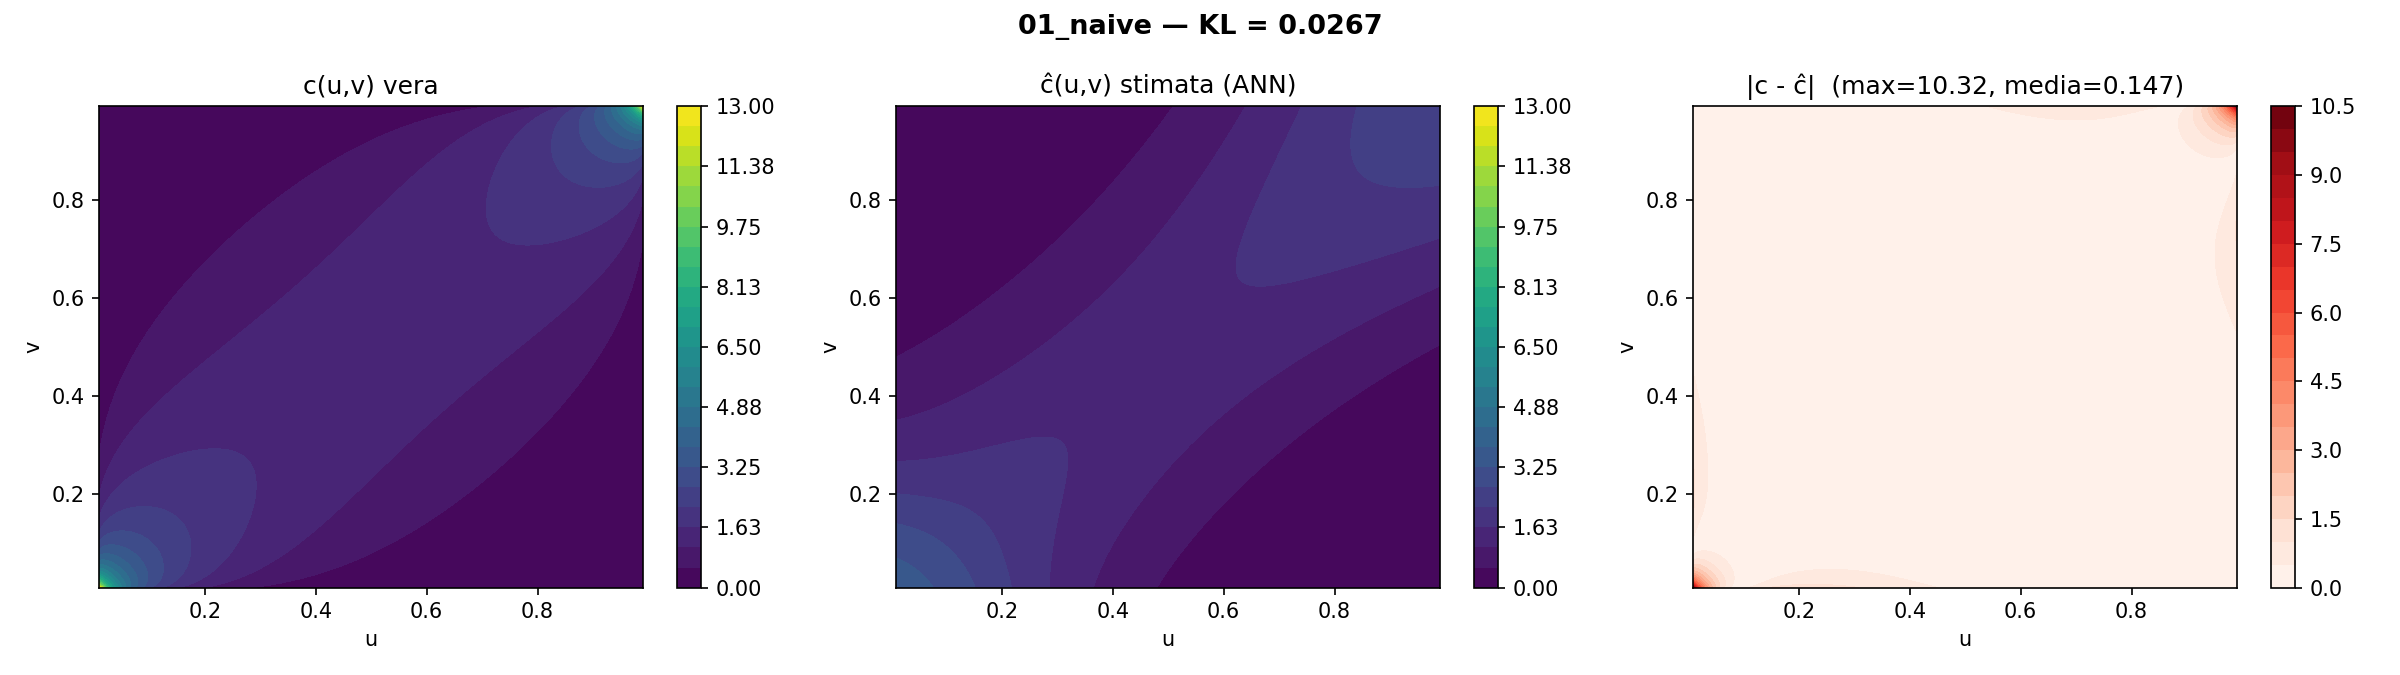
\includegraphics[width=\textwidth]{../plots/01_naive_confronto.png}
\caption{Configurazione naive: confronto tra densità vera (sinistra), stimata (centro) e errore assoluto (destra). La forma qualitativa è catturata, ma la rete fatica a riprodurre i picchi negli angoli $(0,0)$ e $(1,1)$.}
\label{fig:naive_confronto}
\end{figure}

\begin{figure}[ht]
\centering
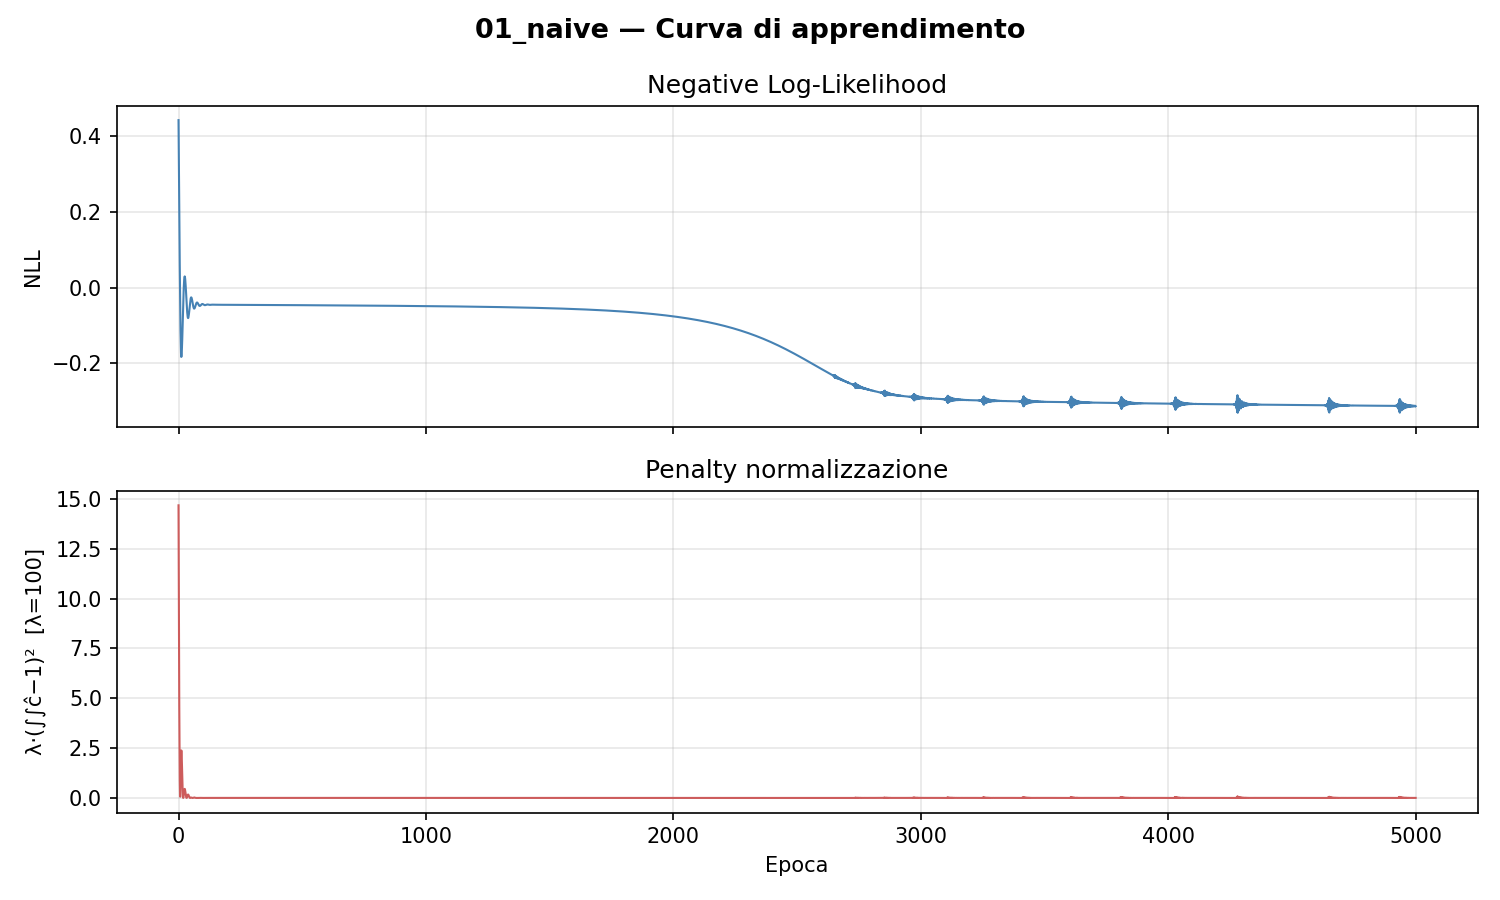
\includegraphics[width=0.85\textwidth]{../plots/01_naive_learning.png}
\caption{Curva di apprendimento --- configurazione naive. In alto: la NLL scende lentamente e mostra un plateau prolungato nelle prime 2000 epoche, indice di un $\lambda$ troppo forte che penalizza l'esplorazione. In basso: il penalty di normalizzazione crolla rapidamente a zero ($\lambda = 100$ forza $\iint \hat{c} \approx 1$ quasi subito), ma a scapito della capacità della rete di imparare la forma.}
\label{fig:naive_learning}
\end{figure}

\subsection{Osservazioni}

\begin{itemize}
    \item La forma qualitativa della copula è catturata (densità alta lungo la diagonale concordante).
    \item L'errore è concentrato agli angoli, dove la densità vera diverge: è un limite intrinseco di un MLP con attivazione \texttt{softplus}.
    \item Il valore alto di $\lambda = 100$ forza una normalizzazione quasi perfetta ($\iint \hat{c} \approx 1.005$), ma rallenta drasticamente la discesa della NLL: la rete dedica troppo budget di ottimizzazione al vincolo e poco alla forma.
\end{itemize}

% =========================================================================
\section{Grid Search}
% =========================================================================

Per trovare la combinazione migliore di iperparametri, abbiamo eseguito una ricerca esaustiva su 24 configurazioni, tutte addestrate per 5000 epoche sullo stesso dataset ($N=2000$, seed fissato per riproducibilità).

\subsection{Spazio di ricerca}

\begin{center}
\begin{tabular}{lll}
\toprule
\textbf{Iperparametro} & \textbf{Valori testati} & \textbf{Ruolo} \\
\midrule
Neuroni/strato (\textit{hidden}) & 32, 64, 128 & Capacità espressiva \\
Strati nascosti (\textit{layers}) & 2, 3 & Profondità della rete \\
$\lambda$ & 10, 100 & Peso del vincolo di normalizzazione \\
Learning rate & $10^{-3}$, $5 \times 10^{-4}$ & Velocità di convergenza \\
\bottomrule
\end{tabular}
\end{center}

\subsection{Top 5 risultati}

\begin{center}
\begin{tabular}{cccccc}
\toprule
\textbf{\#} & \textbf{Hidden} & \textbf{Layers} & $\boldsymbol{\lambda}$ & \textbf{LR} & $\boldsymbol{D_\mathrm{KL}}$ \\
\midrule
1 & 128 & 3 & 10 & $10^{-3}$ & 0.0069 \\
2 & 64  & 2 & 10 & $10^{-3}$ & 0.0077 \\
3 & 128 & 2 & 10 & $5\!\times\!10^{-4}$ & 0.0079 \\
4 & 64  & 3 & 10 & $10^{-3}$ & 0.0080 \\
5 & 128 & 3 & 10 & $5\!\times\!10^{-4}$ & 0.0081 \\
\bottomrule
\end{tabular}
\end{center}

\subsection{Analisi}

Il risultato più netto del grid search è che \textbf{$\lambda = 10$ domina sistematicamente $\lambda = 100$}. Tutte le top 5 configurazioni usano $\lambda = 10$. L'interpretazione è coerente con quanto osservato nell'esperimento naive: un $\lambda$ troppo alto satura il budget di ottimizzazione sul vincolo di normalizzazione, impedendo alla rete di modellare con precisione la forma della densità.

Il learning rate standard ($10^{-3}$) risulta sufficiente. La profondità (3 strati) e la larghezza (128 neuroni) aiutano, ma il guadagno rispetto a configurazioni più piccole è modesto.

% =========================================================================
\section{Esperimento 2: Best configuration}
% =========================================================================

\subsection{Setup}

\begin{center}
\begin{tabular}{ll}
\toprule
\textbf{Parametro} & \textbf{Valore} \\
\midrule
Architettura & MLP: $2 \to 128 \to 128 \to 128 \to 1$ (\texttt{tanh} + \texttt{softplus}) \\
Parametri & 33\,537 \\
$\lambda$ & 10 \\
Learning rate & $10^{-3}$ (Adam) \\
Epoche & 5\,000 \\
$N$ campioni & 2\,000 \\
\bottomrule
\end{tabular}
\end{center}

\subsection{Risultati}

\begin{center}
$D_{\mathrm{KL}} = 0.0142$, \quad errore medio $= 0.154$, \quad $\displaystyle\iint \hat{c}\,du\,dv \approx 1.047$
\end{center}

\begin{figure}[ht]
\centering
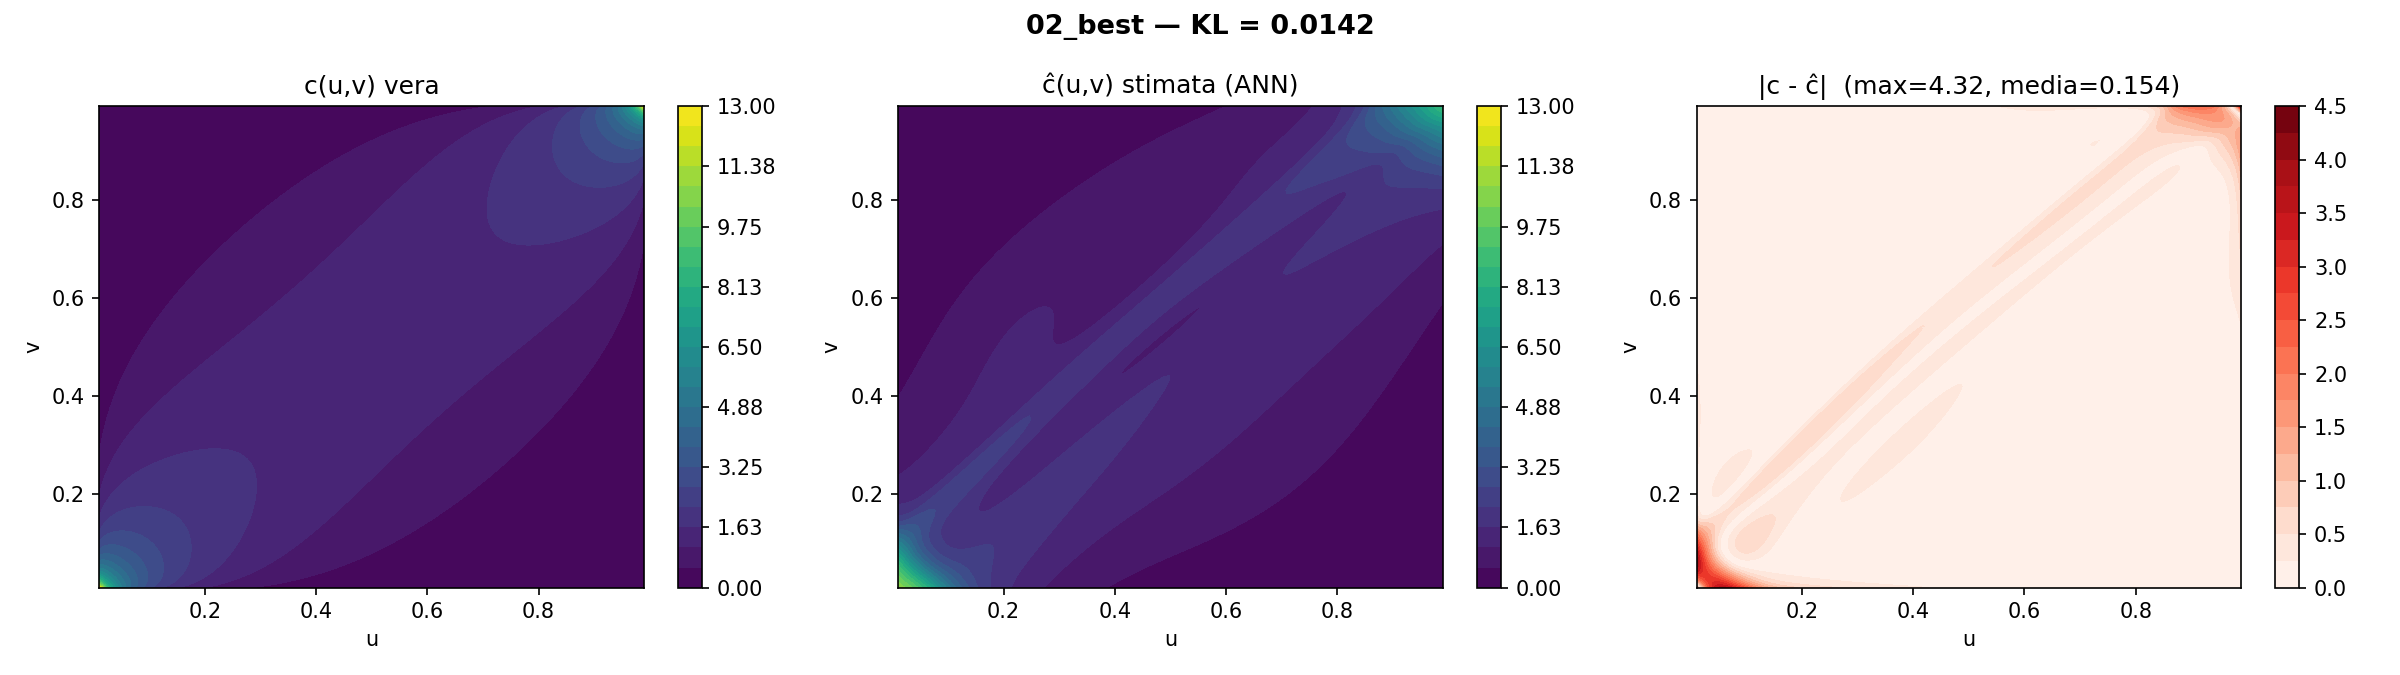
\includegraphics[width=\textwidth]{../plots/02_best_confronto.png}
\caption{Best configuration: il pattern di errore è più strutturato (concentrato lungo la diagonale concordante), ma il massimo errore è sceso da 10.32 a 4.32. La rete sta modellando meglio i picchi.}
\label{fig:best_confronto}
\end{figure}

\begin{figure}[ht]
\centering
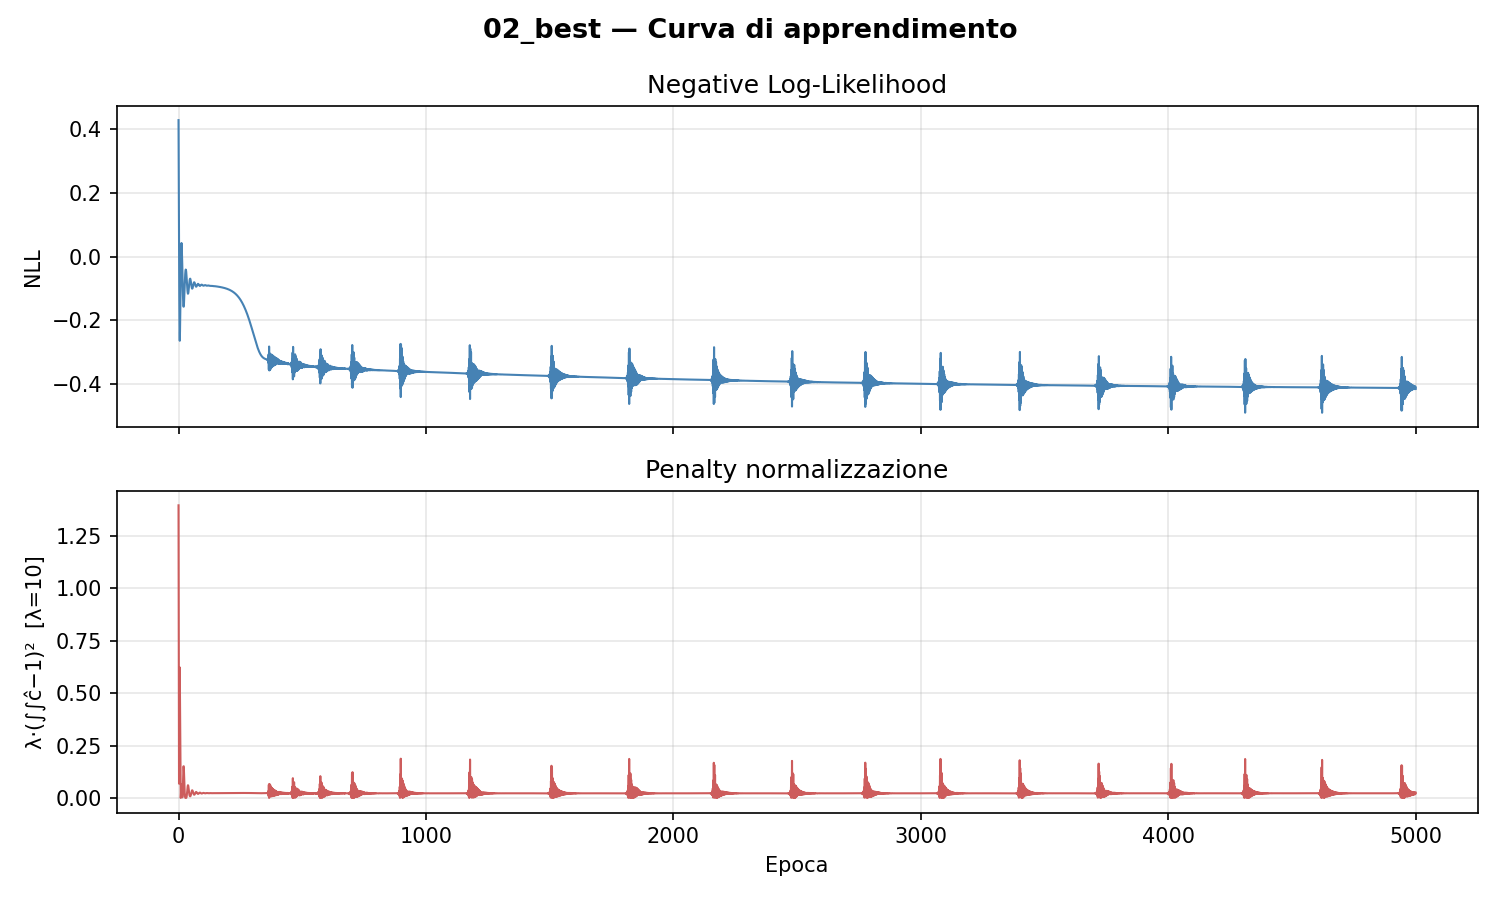
\includegraphics[width=0.85\textwidth]{../plots/02_best_learning.png}
\caption{Curva di apprendimento --- best configuration. La NLL converge molto più rapidamente (raggiunge $-0.35$ entro 500 epoche vs.\ 2500 per la naive) e scende più in basso ($-0.41$ vs.\ $-0.31$). Il penalty oscilla intorno a $0.02$, coerente con $\iint \hat{c} \approx 1.047$.}
\label{fig:best_learning}
\end{figure}

\subsection{Confronto}

\begin{center}
\begin{tabular}{lccc}
\toprule
& $D_{\mathrm{KL}}$ & Errore max & $\iint \hat{c}$ \\
\midrule
Naive ($64 \times 2$, $\lambda\!=\!100$)  & 0.0267 & 10.32 & 1.005 \\
Best ($128 \times 3$, $\lambda\!=\!10$) & 0.0142 & 4.32  & 1.047 \\
\bottomrule
\end{tabular}
\end{center}

La configurazione best dimezza quasi la KL divergence e riduce il picco di errore da 10.32 a 4.32. Il compromesso è un integrale leggermente meno preciso (1.047 vs.\ 1.005), ma accettabile.

% =========================================================================
\section{Prossimi passi}
% =========================================================================

\begin{enumerate}
    \item \textbf{Copula non banale:} testare su una copula con struttura di dipendenza diversa (es.\ Clayton, Gumbel) per verificare la generalizzazione dell'approccio.
    \item \textbf{Dataset reale:} applicare la pipeline a dati reali bivariati (es.\ ritorni finanziari) dove la vera copula è ignota.
    \item \textbf{Confronto con baseline:} KDE bivariata e Gaussian Mixture Models sugli stessi dati, confrontando tramite cross-validation likelihood.
\end{enumerate}

\end{document}
